\documentclass[11pt]{amsbook}

\usepackage{../HBSuerDemir}	% ------------------------

\begin{document}

% ++++++++++++++++++++++++++++++++++++++
\hPage{b1p1/231}
% ++++++++++++++++++++++++++++++++++++++

% ======================================= ENUM START
\begin{hEnumerateArabic}

% ======================================= ITEM 1
\stepcounter{enumi}
\item 

\begin{tabular}{p{0pt} p{0.35\textwidth} p{0pt} p{0.35\textwidth}}
	\vspace{0pt} a)
	&
	\vspace{0pt} 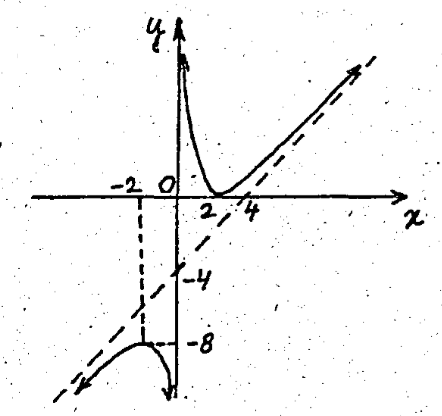
\includegraphics[width=0.35\textwidth]{images/b1p1-231-fig01}
	&
	\vspace{0pt} b)
	&
	\vspace{0pt} 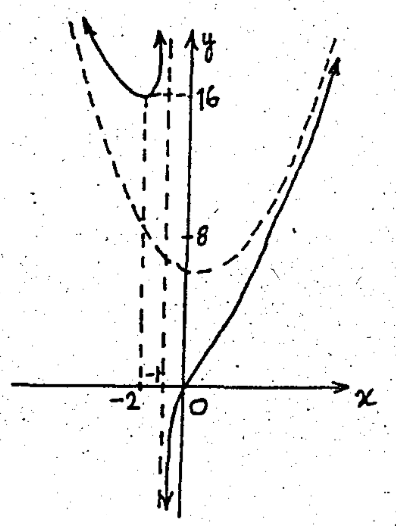
\includegraphics[width=0.35\textwidth]{images/b1p1-231-fig02}
	
	\\

	\vspace{0pt} c)
	&
	\vspace{0pt} 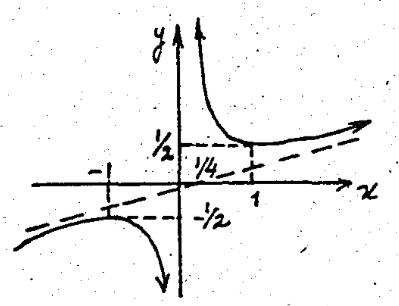
\includegraphics[width=0.35\textwidth]{images/b1p1-231-fig03}
	&
	\vspace{0pt} d)
	&
	\vspace{0pt} 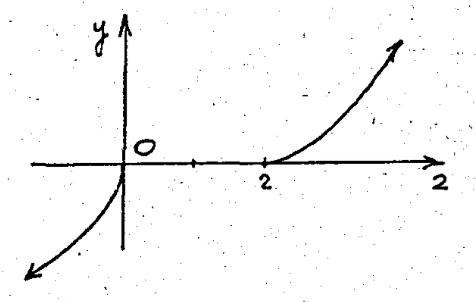
\includegraphics[width=0.35\textwidth]{images/b1p1-231-fig04}
\end{tabular}
\\

% ======================================= ITEM 2
\stepcounter{enumi}
\item The curve is symmetric with respect to the origin:
\begin{center}
	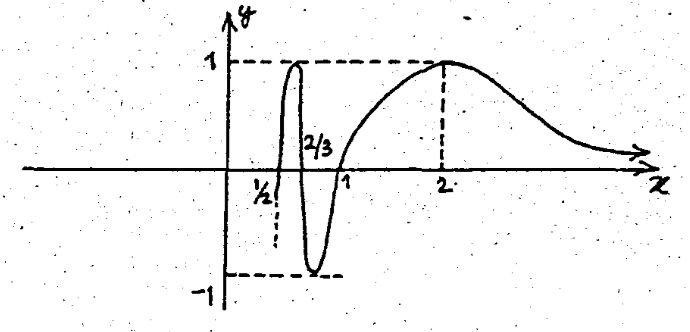
\includegraphics[width=0.5\textwidth]{images/b1p1-231-fig05}
\end{center}

\quad\quad\quad $y = 0$ at $-x = 1/n$ for all $n \in \hSoNp$

\quad\quad\quad $y = 1$ at $x = \frac{2}{2n+1}$ ($n$ even)

\quad\quad\quad $y = {-1}$ at $x = \frac{2}{2n+1}$ ($n$ odd)
\\

% ======================================= ITEM 3
\stepcounter{enumi}
\item a) PCO is an equilateral triangle,\quad b) B 
\\

% ======================================= ITEM 4
\stepcounter{enumi}
\item 4 
\\

% ======================================= ITEM 5
\stepcounter{enumi}
\item $\left(\ell-a\right)\sqrt{\left(\ell^2-a^2\right)/3}$ 
\\

\end{hEnumerateArabic}
% ======================================= ENUM END

\end{document}